
%%%%%%%%%%%%%%%%%%%%%%%%%%%%%%%%%%%%%%%%%%%%%%%%%%%%%%%%%%%%%%%%%%%%%%%%%%%%%%%%%%%%%%%
%%%%%%%%%%%%%%%%%%%%%%%%%%%%%%%%%%%%%%%%%%%%%%%%%%%%%%%%%%%%%%%%%%%%%%%%%%%%%%%%%%%%%%%
% 
% This top part of the document is called the 'preamble'.  Modify it with caution!
%
% The real document starts below where it says 'The main document starts here'.

\documentclass[12pt]{article}

\usepackage{amssymb,amsmath,amsthm}
\usepackage[top=1in, bottom=1in, left=1.25in, right=1.25in]{geometry}
\usepackage{fancyhdr}
\usepackage{enumerate}
\usepackage{listings}
\usepackage{graphicx}
\usepackage{float}
\usepackage{multicol}
% Comment the following line to use TeX's default font of Computer Modern.
\usepackage{times,txfonts}
\usepackage{mwe}
\usepackage{caption}
\usepackage{subcaption}

\usepackage{tikz}
\def\checkmark{\tikz\fill[scale=0.4](0,.35) -- (.25,0) -- (1,.7) -- (.25,.15) -- cycle;} 



\makeatletter
\renewcommand*\env@matrix[1][*\c@MaxMatrixCols c]{%
  \hskip -\arraycolsep
  \let\@ifnextchar\new@ifnextchar
  \array{#1}}
\makeatother

\newtheoremstyle{homework}% name of the style to be used
  {18pt}% measure of space to leave above the theorem. E.g.: 3pt
  {12pt}% measure of space to leave below the theorem. E.g.: 3pt
  {}% name of font to use in the body of the theorem
  {}% measure of space to indent
  {\bfseries}% name of head font
  {:}% punctuation between head and body
  {2ex}% space after theorem head; " " = normal interword space
  {}% Manually specify head
\theoremstyle{homework} 

% Set up an Exercise environment and a Solution label.
\newtheorem*{exercisecore}{\@currentlabel}
\newenvironment{exercise}[1]
{\def\@currentlabel{#1}\exercisecore}
{\endexercisecore}

\newcommand{\localhead}[1]{\par\smallskip\noindent\textbf{#1}\nobreak\\}%
\newcommand\solution{\localhead{Solution:}}

%%%%%%%%%%%%%%%%%%%%%%%%%%%%%%%%%%%%%%%%%%%%%%%%%%%%%%%%%%%%%%%%%%%%%%%%
%
% Stuff for getting the name/document date/title across the header
\makeatletter
\RequirePackage{fancyhdr}
\pagestyle{fancy}
\fancyfoot[C]{\ifnum \value{page} > 1\relax\thepage\fi}
\fancyhead[L]{\ifx\@doclabel\@empty\else\@doclabel\fi}
\fancyhead[C]{\ifx\@docdate\@empty\else\@docdate\fi}
\fancyhead[R]{\ifx\@docauthor\@empty\else\@docauthor\fi}
\headheight 15pt

\def\doclabel#1{\gdef\@doclabel{#1}}
\doclabel{Use {\tt\textbackslash doclabel\{MY LABEL\}}.}
\def\docdate#1{\gdef\@docdate{#1}}
\docdate{Use {\tt\textbackslash docdate\{MY DATE\}}.}
\def\docauthor#1{\gdef\@docauthor{#1}}
\docauthor{Use {\tt\textbackslash docauthor\{MY NAME\}}.}
\makeatother

% Shortcuts for blackboard bold number sets (reals, integers, etc.)
\newcommand{\Reals}{\ensuremath{\mathbb R}}
\newcommand{\Nats}{\ensuremath{\mathbb N}}
\newcommand{\Ints}{\ensuremath{\mathbb Z}}
\newcommand{\Rats}{\ensuremath{\mathbb Q}}
\newcommand{\Cplx}{\ensuremath{\mathbb C}}
%% Some equivalents that some people may prefer.
\let\RR\Reals
\let\NN\Nats
\let\II\Ints
\let\CC\Cplx

%\textbf{Code:}
%\begin{center}
%  \lstinputlisting{NewtonsMethodP5.m}
%\end{center}
%
%\textbf{Console:}
%\begin{center}
%  \lstinputlisting{P5C.txt}
%\end{center}
%\vspace{.15in}


%\begin{figure}[H]
%  \begin{center}
%    \caption{The one-norm unit ball}
%    \includegraphics[width=.76\textwidth]{1norm.png}
%  \end{center}
%\end{figure}




%%%%%%%%%%%%%%%%%%%%%%%%%%%%%%%%%%%%%%%%%%%%%%%%%%%%%%%%%%%%%%%%%%%%%%%%%%%%%%%%%%%%%%%
%%%%%%%%%%%%%%%%%%%%%%%%%%%%%%%%%%%%%%%%%%%%%%%%%%%%%%%%%%%%%%%%%%%%%%%%%%%%%%%%%%%%%%%
% 
% The main document start here.

% The following commands set up the material that appears in the header.
\doclabel{Math 615: Homework 2}
\docauthor{Stefano Fochesatto}
\docdate{\today}


\begin{document}


\begin{exercise}{Problem P7} Suppose this table of 'data' give samples of the function $Z(h)$:
  \begin{center}
    \begin{tabular}{ l |l| l| l| l| l |l}
    h& 1.0 &0.5& 0.1& 0.05& 0.01 & 0.005\\
    \hline
    Z(h)& 28.43 &10.747& 0.5540& 0.5555& 0.04849 & 0.005521
    \end{tabular}
    \end{center}
  
  This data may be fitted by a function $f(h) = Ch^p$ for some values $C$ and $p$. Find these values by 
  fitting a straight line to the logarithms of the data; in Matlab you may use polyfit. Then graph the data and show the 
  fitted line on the same axes, using Matlab's loglog or similar.
  \solution Let $ln(f(x))$ be the linear regression fitted to the log transformed data, 
  \begin{equation*}
    ln(f(x)) = x_1 (ln(h)) + x_0
  \end{equation*}
  Solving $f(x)$ we get the following, 
  \begin{align*}
    ln(f(x)) &= x_1 (ln(h)) + x_0,\\
    ln(f(x)) &= ln(h^{x_1}) + x_0,\\
    e^{ln(f(x))} &= e^{ln(h^{x_1}) + x_0},\\
    f(x) &= e^{x_0}e^{ln(h^{x_1})},\\
    f(x) &= e^{x_0}h^{x_1}.
  \end{align*}
  So $C = e^{x_0}$ and $p = x_1$. The following code fits the linear regression to the log transformed data and 
  generates a loglog plot with the original data. From the code we see that $C \approx 29.8892$ and $p\approx 1.5143$.\\
  \textbf{Console:}
  \begin{center}
    \lstinputlisting[basicstyle=\footnotesize]{r1.txt}
  \end{center}


  \begin{figure}[H]
    \begin{center}
      \caption{Loglog plot of $Z(h)$ with $f(h)$ in red.}
      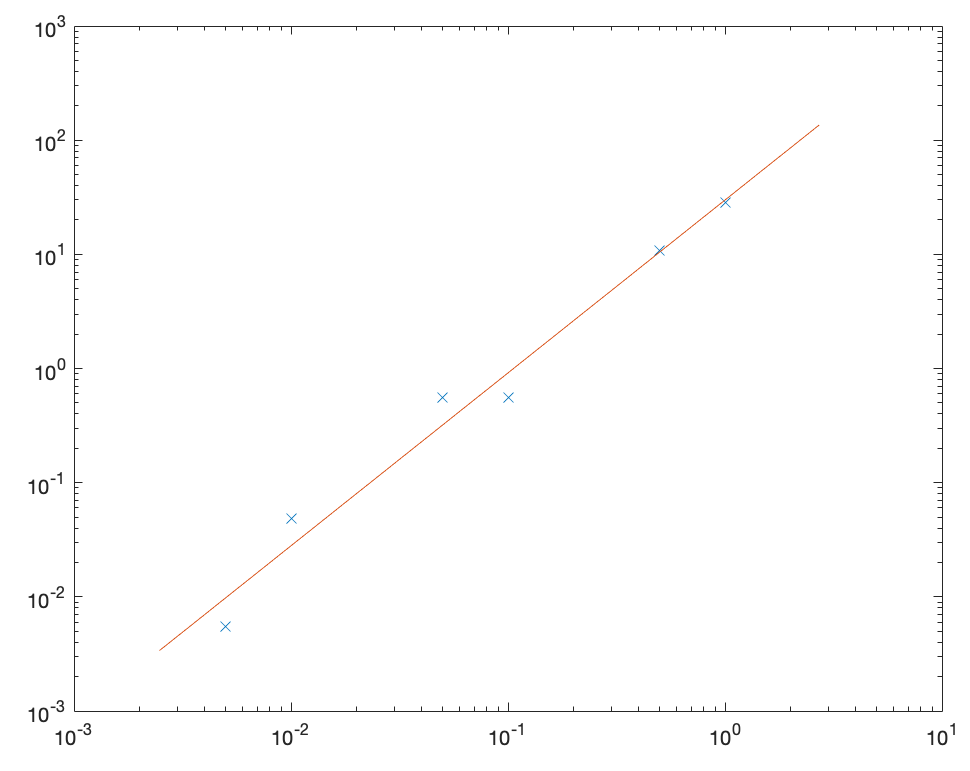
\includegraphics[width=.80\textwidth]{r2.png}
    \end{center}
  \end{figure}

\end{exercise}
\vspace{1in}

  

\begin{exercise}{Problem P8} Reproduce Figure 1.2 on page 6 of the textbook. In particular, write 
  a code which generates the data show in Table 1.1, by doing the calculations described by Example 1.1, 
  with $u(x) = \sin(x)$ and $\overline{x} = 1$. Then generate the Figure, which has logarithmic scaling on both 
  axes. 
  \solution 

  \textbf{Code:}
  \begin{center}
    \lstinputlisting[basicstyle=\footnotesize]{r2.txt}
  \end{center}

  \begin{figure}[H]
    \begin{center}
      \caption{Loglog plot of Error in Various FD Approx.}
      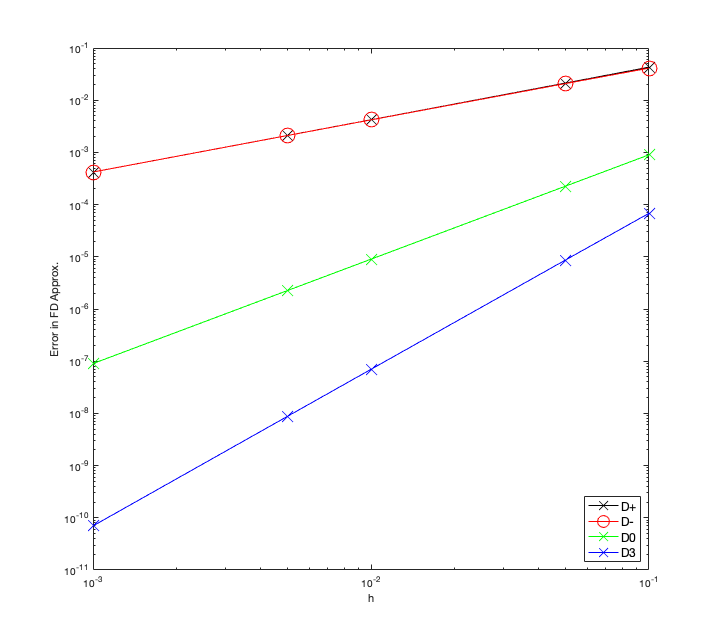
\includegraphics[width=.80\textwidth]{r3.png}
    \end{center}
  \end{figure}

  
\end{exercise}
\vspace{1in}




\begin{exercise}{Problem P9}
  \begin{enumerate}
    \item[(a)] Use the method of undetermined coefficient to set up a $5 x 5$ linear system that 
    determine the fourth-order centered finite difference approximation to $u''(x)$ based on 5 equally 
    spaced points, namely
    \begin{equation*}
      u''(x) = c_{-2}u(x - 2h) + c_{-1}u(x - h) + c_0u(x) + c_{1}u(x + h) + c_{2}u(x + 2h) + O(h^4)
    \end{equation*}
    In particular, expand $u(x - 2h), u(x - h), u(x + h), u(x + 2h)$ in Taylor series. Then collect terms on the 
    right side of the above equation to generate a square linear system $Ac = g$ in unknowns $c_{-2},c_{-1}, c_{0}, c_{1}, c_{2}$.
    This system will have numerical entries in the matrix $A$, but the entries of vector $G$ will depend on $h$.
    \solution Applying Taylor's Theorem we can expand each function $u(x - 2h), u(x - h), u(x + h)$ and $u(x + 2h)$
    in terms of $u(x)$ and it's derivatives. Doing so to the fourth order we get the following, 
    \begin{align*}
      u(x - 2h) &= u(x) - 2hu'(x) + \frac{1}{2}(2h)^2u''(x) - \frac{1}{6}(2h)^3u'''(x) + \frac{1}{24}(2h)^4u''''(x) + O(h^5),\\
      u(x - h) &= u(x) - hu'(x) + \frac{1}{2}h^2u''(x) - \frac{1}{6}h^3u'''(x) + \frac{1}{24}h^4u''''(x) +  O(h^5),\\
      u(x + h) &= u(x) + hu'(x) + \frac{1}{2}h^2u''(x) + \frac{1}{6}h^3u'''(x) +  \frac{1}{24}h^4u''''(x) + O(h^5),\\
      u(x + 2h) &= u(x) + 2hu'(x) + \frac{1}{2}(2h)^2u''(x) + \frac{1}{6}(2h)^3u'''(x) + \frac{1}{24}(2h)^4u''''(x)+ O(h^5).
    \end{align*}
    By substitution and collecting like terms we get the following, 
    \begin{align*}
      D^2_4(x) &= (c_{-2} + c_{-1} + c_0 + c_1 + c_2)u(x)\\
              &+ (-2c_{-2} - c_{-1} + c_1 + 2c_2)hu'(x)\\
              &+ (2c_{-2} + \frac{1}{2}c_{-1} + \frac{1}{2}c_{1} + 2c_{2})h^2u''(x)\\
              &+ \left(-\frac{4}{3}c_{-2} - \frac{1}{6}c_{-1} + \frac{1}{6}c_1 + \frac{4}{3}c_{2}\right)h^3u'''(x)\\
              &+ \left(\frac{1}{6} + \frac{1}{24} + 0 + \frac{1}{24} + \frac{1}{6}\right)h^4u''''(x)\\
              &+ O(h^5).
    \end{align*}
    By method of undetermined coefficient we get the following system of equations. 
    \begin{equation*}
      \begin{bmatrix}
        1 & 1 & 1 & 1 & 1 \\
        -2 & -1 & 0 & 1 & 2\\
        2 & \frac{1}{2}& 0 &\frac{1}{2}&2\\
        -\frac{4}{3}& -\frac{1}{6}&0&\frac{1}{6} & \frac{4}{3}\\
        \frac{2}{3} & \frac{1}{24} & 0 & \frac{1}{24}&\frac{2}{3}
      \end{bmatrix}
      \begin{bmatrix}
        c_{-2}\\
        c_{-1}\\
        c_{0}\\
        c_{1}\\
        c_{2}
      \end{bmatrix}
      = 
      \begin{bmatrix}
        0\\
        0\\
        \frac{1}{h^2}\\
        0\\
        0
      \end{bmatrix}
    \end{equation*}

    \item[(b)] Use Matlab to solve the linear system from part $(a)$. A recommended way to do this is 
    to use $h = 1$ in the vector $g$ and solve the system numerically using the 'backslash' method. Then
    write down the answer in the form like $(1.11)$, inserting the correct power of $h$. Use $h = .5$ 
    to confirm that that you've captured the correct powers. 
    \solution Solving the system numerically we get the following finite difference approximation, 
    \begin{equation*}
      D^2_5(x) = \frac{1}{h^2}\left[-\frac{1}{12}u(x - 2h) + \frac{4}{3}u(x - h) - \frac{5}{2}u(x) + \frac{4}{3}u(x + h) -\frac{1}{12}u(x + 2h)\right].
    \end{equation*}
    As suggested we solved the system numerically with $h = 1$, put the approximation in the form of $(1.11)$ then solved with $h = .5$, comparing the results to 
    see that we must divide the coefficients by a factor of $1/h^2$. \\


    \textbf{Console:}
    \begin{center}
      \lstinputlisting[basicstyle=\footnotesize]{r3.txt}
    \end{center}
  \end{enumerate}
\end{exercise}
\vspace{1in}


\begin{exercise}{Problem P10} In Section $2.4$ the textbook uses finite differences to convert the boundary
  value problem, 
  \begin{equation*}
    u''(x) = f(x), \qquad u(0) = \alpha, \qquad u(1) = \beta
  \end{equation*}
  into matrix equation $AU = F$, with $A$ and $F$ given in (2.10). For any integer $m \geq 1$, 
  this method is based on a grid with $h = 1/(m + 1)$ and $x_j = jh$. There are $m$ unknowns
  $U_1, U_2, \dots, U_m$ located at the interior nodes $x_1,\dots, x_m$. Note that finite difference 
  approximation $D^2$ from equation $(1.13)$ is used for the $u''$ term. 
  
  Assume $q, x_L, x_R$ are real numbers with $x_L < x_R$. Similar to the method in Section 2.4, 
  create a finite difference approximation for the problem
  \begin{equation*}
    u''(x) + qu(x) = f(x),\qquad u(x_L) = \alpha,\qquad u(x_R) = \beta
  \end{equation*} 
  Use the same approximation $D^2$ for $u''$. Use the same grid indexing with $m$ unknowns $U_1, \dots,U_m$
  and give the new formulas for $x_j$ and the mesh width $h$. State, in detail, $A$ and $F$ in $AU = F$
  \solution 
  First note that a grid with $m + 2$ indices across an interval from $x_L$ to $x_R$ will have
  $m-1$ spaces, each with size $h = (x_R - x_L)/(m - 1)$.
  Our formula for each $x_j$ is given by $x_j = jh + x_L$. 
    Recall that the finite difference approximation for $D^2$ used in $(1.13)$ goes as follows, 
  \begin{equation*}
    D^2U_j = \frac{1}{h^2}\left(U_{j - 1} -2U_j + U_{j + 1}\right).
  \end{equation*}
  By substitution we get the following set of equations, 
  \begin{equation*}
    \frac{1}{h^2}\left(U_{j - 1} -2U_j + U_{j + 1}\right) + qU_j = f(x_j) \qquad \text{for } j = 1, 2,\dots, m.
  \end{equation*}
  Written out with matrix notation we get the following, 
  \begin{equation*}
    A = \frac{1}{h^2}
    \begin{bmatrix}
         (qh^2 - 2) &    1    &         &         &         &         \\ 
               1 & (qh^2 - 2) &    1    &         &         &         \\ 
                 &    1    & (qh^2 - 2) &    1    &         &         \\ 
                 &         &  \ddots &  \ddots & \ddots  &         \\
                 &         &         &    1    & (qh^2 - 2) &   1     \\
                 &         &         &         &    1    & (qh^2 - 2) 
    \end{bmatrix}, 
    \qquad
    F = 
    \begin{bmatrix}
      f(x_1) - \alpha/h^2  \\ 
      f(x_2)               \\ 
      f(x_3)               \\ 
      \vdots               \\
      f(x_{m - 1})         \\
      f(x_m) - \beta/h^2  
    \end{bmatrix}.
  \end{equation*}  
\end{exercise}
\vspace{1in}



\begin{exercise}{Problem P11} Continuing along the lines of $P10$, setup a finite difference method for 
  the most general linear, second-order Dirichlet boundary value problems:
  \begin{equation*}
    u''(x) + p(x)u'(x) + q(x)u(x) = f(x), \qquad u(x_L) = \alpha, \qquad u(x_R) = \beta.
  \end{equation*}
  Compared to $P10$, now $p(x)$, $q(x)$ are arbitrary function like $f(x)$. Use approximation(1.3), 
  namely the centered finite difference $D_0$, for the $u'$ term. State $A$ and $F$ in the linear system $AU = F$.
  \solution First note that our grid scheme is the same as $P10$ with $h = (x_R - x_L)/(m - 1)$ for spacing and $x_j = jh + x_L$ for each point. 
  Recall the centered finite difference scheme approximation for $u'$,   
  \begin{equation*}
    D_0U_j = \frac{1}{2h}\left(U_{j + 1} - U_{j - 1}\right).
  \end{equation*}
  Using the same finite difference approximation for $D^2$ as in the last problem, by substitution we get the following set of equations, 
  \begin{equation*}
    \frac{1}{h^2}\left(U_{j - 1} -2U_j + U_{j + 1}\right) + p(x_j)\frac{1}{2h}\left(U_{j + 1} - U_{j - 1}\right) + q(x_j)U_j = f(x_j), \quad \text{for } j = 1, 2,\dots, m.
  \end{equation*}
  Through some algebra and combining like terms we get, 
  \begin{align*}
    \frac{1}{h^2}\left(U_{j - 1} -2U_j + U_{j + 1}\right) + p(x_j)\frac{1}{2h}\left(U_{j + 1} - U_{j - 1}\right) + q(x_j)U_j &= f(x_j)\\
    \frac{1}{h^2}\left(U_{j - 1} -2U_j + U_{j + 1} + \frac{p(x_j)h}{2}\left(U_{j + 1} - U_{j - 1}\right) + q(x_j)h^2U_j\right) &= f(x_j)\\
    \frac{1}{h^2} \left( \left(1 - \frac{p(x_j)h}{2}\right)U_{j-1} + \left(q(x_j)h^2 - 2\right)U_j + \left(1 + \frac{p(x_j)h}{2}\right)U_{j+1} \right) &= f(x_j).
  \end{align*}
  Written out with matrix notation we get, 
  
  \begin{equation*}
    A = \frac{1}{h^2}
    \begin{bmatrix}
         (q(x_1)h^2 - 2) &   \left(1 + \frac{p(x_1)h}{2}\right)    &         &         &                  \\
         \left(1 - \frac{p(x_2)h}{2}\right)   & (q(x_2)h^2 - 2) &    \left(1 + \frac{p(x_2)h}{2}\right)   &         &                  \\ 
                 &    \ddots    & \ddots &    \ddots    &            \\ 
                          &         &      \left(1 - \frac{p(x_{m - 1})h}{2}\right)    & (q(x_{m-1})h^2 - 2)  &   \left(1 + \frac{p(x_{m - 1})h}{2}\right)     \\
                          &         &         &      \left(1 - \frac{p(x_m)h}{2}\right)    & (q(x_m)h^2 - 2) 
    \end{bmatrix}
  \end{equation*}


  \begin{equation*}
    F = 
    \begin{bmatrix}
      f(x_1) - \frac{1}{h^2}\left(1 - \frac{p(x_L)h}{2}\right)\alpha  \\ 
      f(x_2)               \\ 
      f(x_3)               \\ 
     \vdots               \\
      f(x_{m - 1})         \\
      f(x_m) - \frac{1}{h^2}\left(1 + \frac{p(x_R)h}{2}\right)\beta 
    \end{bmatrix}.
  \end{equation*}
  
\end{exercise}


\end{document}
















